\documentclass[a4paper,12pt]{ujarticle}

% upLaTeX用の日本語パッケージ
\usepackage[utf8]{inputenc}
\usepackage{otf}
\usepackage{amsmath,amssymb,amsfonts}
\usepackage{graphicx}
\usepackage[dvips]{color}
\usepackage{url}
\usepackage{geometry}
\geometry{margin=2.5cm}

% 画像パス設定
\graphicspath{{./}{../}}

% タイトル設定
\title{upLaTeX用サンプル文書}
\author{テスト作成者}
\date{\today}

\begin{document}

\maketitle

\section{はじめに}

これはupLaTeXの自動ビルド機能をテストするために作成されたサンプル文書です。

\section{数式}

簡単な数式の例:
\begin{equation}
    E = mc^2
\end{equation}

インライン数式の例: $\int_{-\infty}^{\infty} e^{-x^2} dx = \sqrt{\pi}$

\section{リスト}

\subsection{箇条書き}
\begin{itemize}
    \item 第一項目
    \item 第二項目
    \item 第三項目
\end{itemize}

\subsection{番号付きリスト}
\begin{enumerate}
    \item 最初の手順
    \item 二番目の手順
    \item 三番目の手順
\end{enumerate}

\section{表}

\begin{table}[h]
    \centering
    \begin{tabular}{|c|c|c|}
        \hline
        列1 & 列2 & 列3 \\
        \hline
        A  & B  & C  \\
        D  & E  & F  \\
        \hline
    \end{tabular}
    \caption{サンプル表}
    \label{tab:sample}
\end{table}

\section{日本語の特徴}

upLaTeXでは以下のような日本語の特徴を適切に処理できます:

\begin{itemize}
    \item ひらがな、カタカナ、漢字の混在
    \item 句読点の適切な配置
    \item 日本語と英語の混在: Hello World こんにちは世界
    \item 数式との組み合わせ: 円周率は$\pi \approx 3.14159$である
\end{itemize}

% 章ファイル読み込み
\section{upLaTeX実例章}

\subsection{概要}

この章では、upLaTeXにおける画像参照と参考文献管理のベストプラクティスを実装しています。

\subsection{画像参照の実装}

図\ref{fig:test_image_up}に示すテスト画像は、\texttt{graphicspath}による相対パス参照で読み込まれています。

\begin{figure}[htbp]
    \centering
    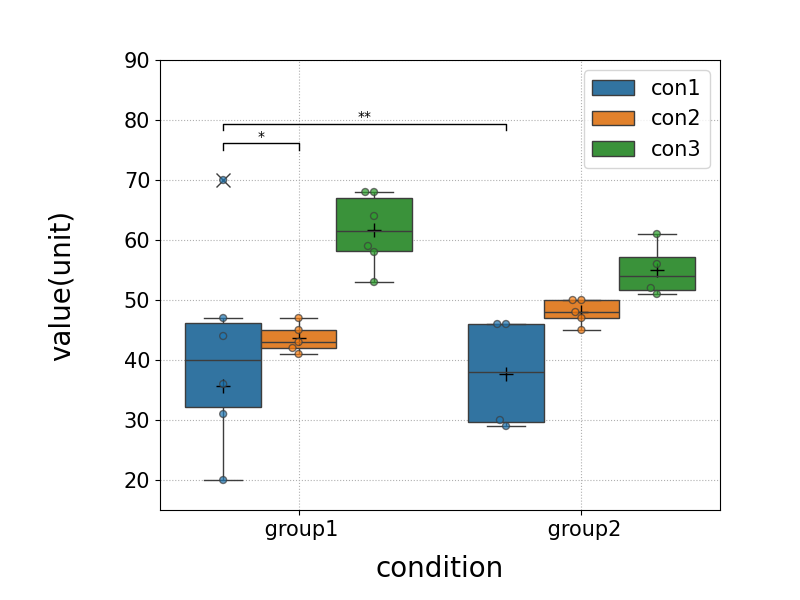
\includegraphics[width=0.7\textwidth,bb=0 0 512 384]{test/test.png}
    \caption{upLaTeX用テスト画像}
    \label{fig:test_image_up}
\end{figure}

upLaTeXでは日本語文字との組み合わせにおいても、適切な画像配置が可能です。

\subsection{文献参照}

参考文献の例として、Doe~\cite{example}による研究を引用します。upLaTeXでは\texttt{pbibtex}により日本語を含む参考文献も適切に処理されます。

\subsection{技術的特徴}

本文書構造では以下の技術的特徴を実装しています:

\begin{itemize}
    \item \texttt{graphicspath}による画像パス自動解決
    \item 相対パス参照による可搬性の確保
    \item \texttt{pbibtex}による日本語対応文献管理
\end{itemize}

\subsection{まとめ}

upLaTeXを使用することで、従来のpLaTeXの利点を保ちながら、UTF-8エンコーディングによる現代的な日本語文書作成が可能になります。


\section{参考文献}

upLaTeXの詳細については、日本語LaTeXの公式ドキュメントを参照してください。

% 参考文献
\bibliographystyle{plain}
\bibliography{reference}

\section{まとめ}

この文書はupLaTeXで正常にコンパイルされ、LaTeX Workshopの自動ビルド機能のテストに使用できます。

\end{document}
